\chapter{Attacchi quantistici alla Proof-of-Stake}
La Blockchain è indiscutibilmente una delle tecnologie più recenti e fiorente degli ultimi dieci anni, se non la tecnologia del futuro. Però a minacciare la sicurezza di quest'utlima è l'ormai incombente crescita di un ulteriore tecnologia: il Quantum Computing.

In particolare ci concentreremo sull'algoritmo di consenso Proof-of-Stake limitando l'attenzione a due noti algoritmi quantistici, quello di Grover e quello di Shor. Questi due algoritmi, come vedremo, possono risolvere alcuni problemi in tempi considerevolmente minori rispetto alle controparti tradizionali, dando quindi la possibilità di violare schemi di crittografia a chiave pubblica.

\section{Proof-of-Stake}
All'interno del capitolo \ref{chap:blockchain} abbiamo già introdotto parte dell'algoritmo di consenso in questione che però andremo ad approfondire all'interno di questo capitolo, cercando di illustrare qual è il razionale che c'è dietro questa scelta.

\subsection{Cos'è una Proof-of-Stake?}
È detto Proof-of-Stake un tipo di protocollo per la messa in sicurezza di una rete di criptovaluta e per il conseguimento di un consenso distribuito. È basato sul principio che a ogni utente venga richiesto di dimostrare il possesso di un certo ammontare di criptovaluta. Si differenzia dai sistemi Proof-of-Work che sono basati su algoritmi di hash che validano le transazioni elettroniche.

\subsection{Utilizzatori}
\textit{Peercoin} è stata la prima criptovaluta ad introdurre sin dal lancio il sistema Proof of Stake senza mai implementarlo completamente. Altre note implementazioni del PoS sono \textit{BitShares}, \textit{Nxt}, \textit{GridCoin}, \textit{BlackCoin} e \textit{Cardano}.

\subsection{Vantaggi, svantaggi e critiche}
Il PoS viene considerato il meccanismo di consenso più decentralizzato, richiede minori barriere tecniche per partecipare alla rete, i nodi sono più distribuiti e di conseguenza la sicurezza è maggiore. Una critica che viene mossa al PoS è quella di avvantaggiare i grandi holder che, avendo più criptovalute in staking, vengono selezionati più spesso per validare i blocchi e guadagnare gli incentivi. Tuttavia la grandezza dello stake è un incentivo a svolgere il lavoro di validazione correttamente e frequentemente. Più la posta in gioco è alta, più alto è il rischio di perderla quando si commettono degli errori nella validazione.

La Proof-of-Work si basa sul consumo di energia: ciò significa che un bene tangibile esterno mette in sicurezza la rete. Di contro, questo porta ad un consumo sempre maggiore di energia. Invece, le criptovalute basate sulla Proof-of-Stake possono essere migliaia di volte più efficienti. Questi costi di mining esercitano la funzione di calmierare il prezzo della valuta.

\section{Modelli di attacco}
Nonostante la Blockchain sia considerata una delle tecnologie più all'avanguardia dell'ultimo decennio, se non la tecnologia del futuro, a minacciare la sua sicurezza è l'ormai rilevante crescita di un'ulteriore innovativa e fiorente tecnologia: il Quantum Computing. In particolare, algoritmi quantistici, come l'algoritmo di fattorizzazione di Shor e l'algoritmo di ricerca di Grover, possono risolvere alcuni problemi in tempi considerevolmente minori rispetto alla loro corrispondente classica, dando quindi la possibilità ai computer quantistici di violare, utilizzando migliaia di qubit, schemi di crittografia a chiave pubblica, come RSA ed Elliptic Curve, che sono alla base della sicurezza dei sistemi come la Blockchain.

È proprio per questo motivo che il NIST, National Institute of Standards and Technology, ha iniziato un processo di ricerca, valutazione e standardizzazione di uno o più algoritmi di cifratura resistenti alla computazione quantistica.

Vediamo di seguito le principali modalità di attacco alla Blockchain.

\subsection{Algoritmo di ricerca di Grover}
Ideato nel 1996 da Lov Grover, è un algoritmo di ricerca che, sfruttando l'amplificazione d'ampiezza, è in grado di cercare un elemento o un valore, in un insieme non ordinato, in tempo \(O\left(\sqrt{N}\right)\) a differenza degli algoritmi classici che risolvono lo stesso problema in tempo \(O\left(N\right)\).

\begin{figure}[h]
  \centering
  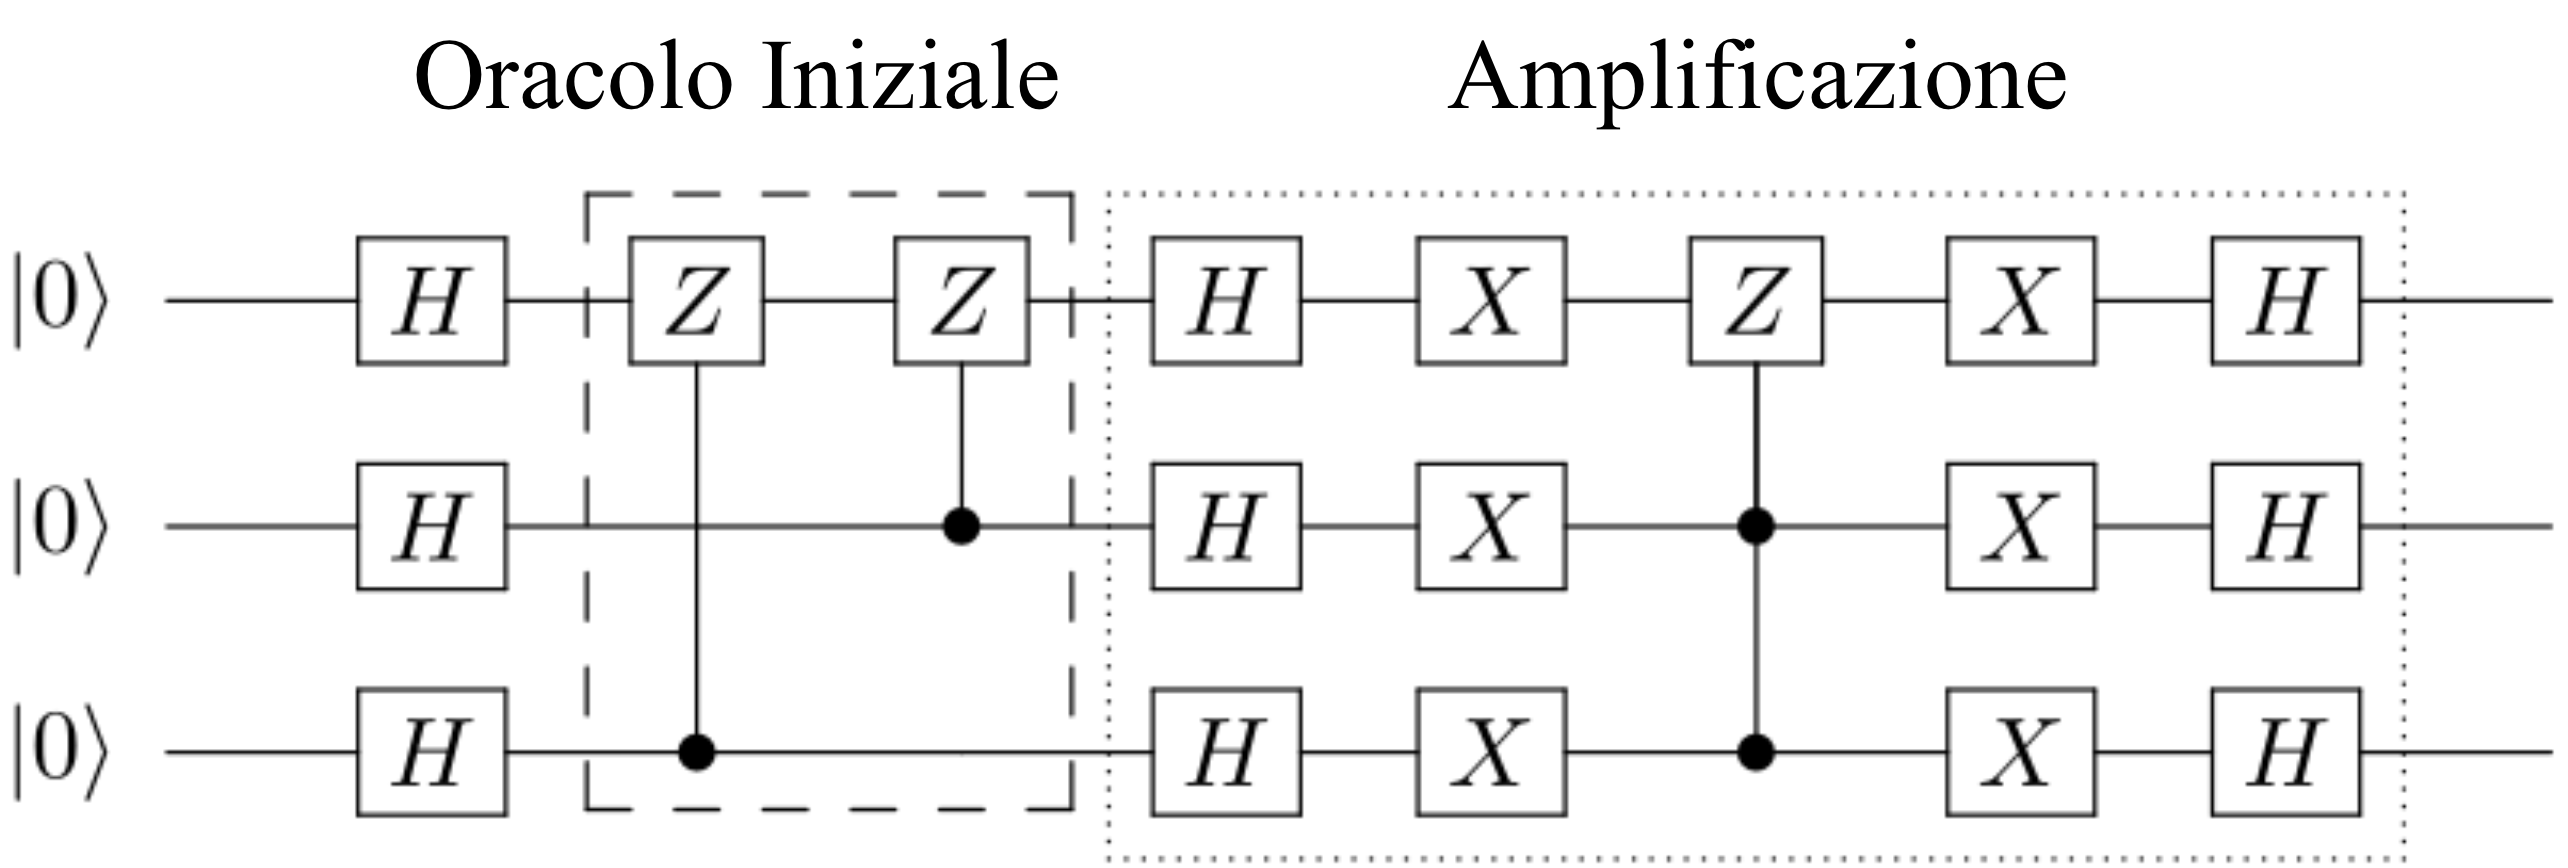
\includegraphics[width=0.7\textwidth]{grover_example.png}
  \caption{Esempio di algoritmo di Glover per 3 qubit}
  \label{fig:grover_example}
\end{figure}

Nei sistemi blockchain, l'algoritmo di Grover fornisce una ricerca più veloce rispetto alle funzioni hash crittografiche utilizzate per generare gli indirizzi degli asset e per proteggere gli hash dei blocchi e delle transazioni.

Andiamo ad analizzare i due passaggi fondamentali dell'algoritmo.
\subsubsection{Funzionamento - Passo 1}
Dato \(n\), un numero necessario per rappresentare uno spazio di ricerca di dimensione \(2^n = N\) tutti inizializzati su \(|0\rangle\), tale che
\[ |0\rangle \otimes n = |0\rangle \]
il primo passo dell'algoritmo di Grover consiste nell'accesso ad un registro di \(n\) qubit. Dobbiamo quindi creare una sovrapposizione uguale di stati, applicando l'operatore Hadmard:
\[ |\psi\rangle = H \otimes n |0\rangle \otimes n = \frac{1}{\sqrt{2^n}} \sum_{x=0}^{2^n} |0\rangle \]

\subsubsection{Funzionamento - Passo 2}
Il secondo passo dell'algoritmo, nonchè anche parte centrale definita come iterazione di Grover, viene ripetuto per un totale di \( \frac{\pi}{4}\sqrt{2^n} \) volte. A sua volta, il secondo passo può essere diviso in due: il primo passo che non è altro che una query quantistica \(\theta\), e il secondo passo definito come trasformazione di diffusione.

\begin{description}
  \item[Oracolo] Definiamo un oracolo quantistico come una "black box", ovvero una scatola nera capace di riconoscere le soluzioni al problema di ricerca e di osservare e modificare il sistema, riconoscendo se è nello stato corretto. Supponiamo di avere uno spazio di ricerca composto da \(N\) elementi etichettati da indici che saranno rappresentati da un valore numerico compreso tra \(0\) e \(N - 1\). Sia \(n\) il numero di bit necessari per rappresentare un indice, poniamo \(N = 2^n\), tale che il numero \(L\) di soluzioni ammesse dalla nostra ricerca sia \(1 \geqslant L \leqslant N\). Definiamo, quindi, una funzione \(f(x)\) con \(x \in [0, N - 1]\) tale che \(f (x) = 1\) se \(x\) è una soluzione al nostro problema mentre \(f(x) = 0\) se \(x\) non è soluzione al nostro problema.
  Tornando quindi al nostro oracolo, definendo \(|q\rangle\) come qubit oracolo e \(|x\rangle\) il nostro indice, allora questo agirà nel seguente modo
  \[ |x\rangle |q\rangle \rightarrow |x\rangle |q \otimes f(x)\rangle \]
  tale che se \(f(x) = 0\), il qubit oracolo resta invariato mentre se \(f(x) = 1\) verrà invertito.
  In sintesi, quindi, l’implementazione dell’oracolo quantistico può essere definita come
  \[ |x\rangle \overset{\theta}{\rightarrow} (-1)^{f(x)} |x\rangle \]
  \item[Trasformata di diffusione] La seconda parte dell'iterazione di Grover, definita come trasformazione di diffusione, consiste in un'ulteriore applicazione dell'operatore Hadmard, in modo tale da avere una sovrapposizione uniforme, seguita da uno spostamento condizionale che sposta ogni stato, escluso \(|0\rangle\), di -1.
  \[ |x\rangle \rightarrow -(-1)^{\delta x 0} |x\rangle \]
  Alla fine, si procede con una seconda applicazione dell'operatore Hadmard. In sintesi, quindi, andando ad includere l'oracolo \(\theta\), l'iterazione di Grover può essere scritta come
  \[ G = (2 | \psi \rangle \langle \psi | - I) \theta \]
\end{description}

\subsection{Algoritmo di fattorizzazione di Shor}
Nel 1994, l'informatico teorico statunitense Peter Shor progetta un efficiente algoritmo quantistico capace di risolvere il problema della fattorizzazione di interi molto grandi in tempo polinomiale e non più in tempo esponenziale.

\begin{figure}[h]
  \centering
  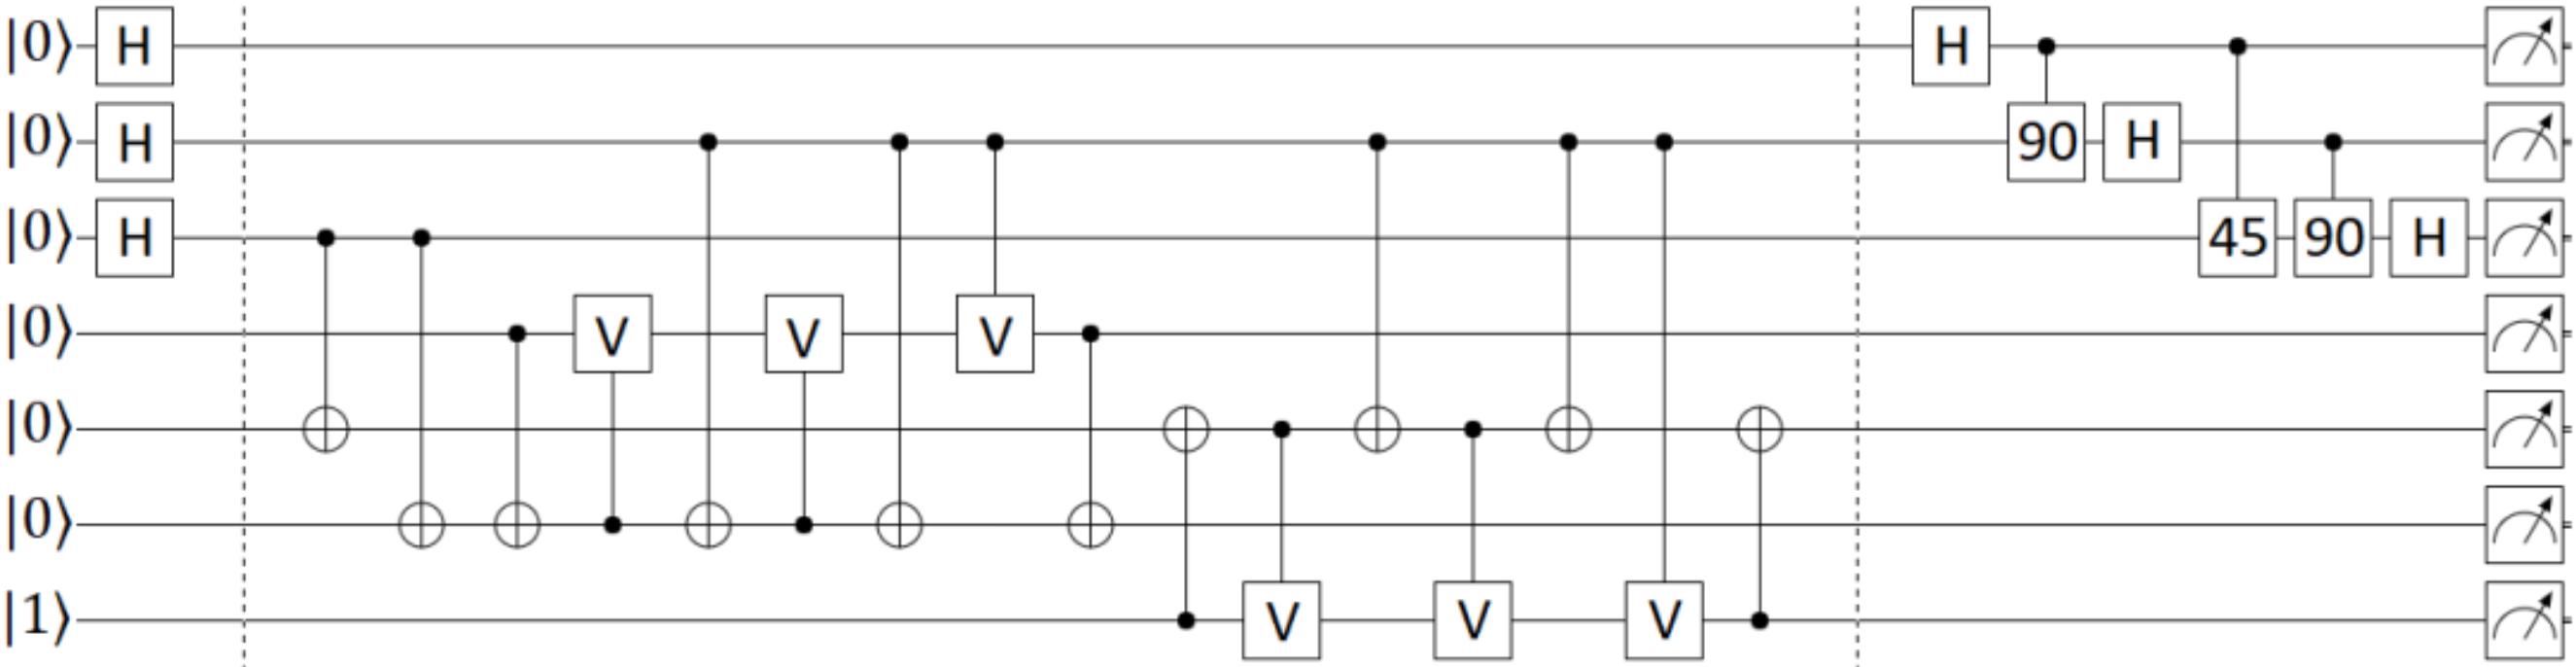
\includegraphics[width=0.7\textwidth]{shor_example.png}
  \caption{Esempio di algoritmo di Shor per fattorizzare il numero 15}
  \label{fig:shor_example}
\end{figure}

\subsubsection{Funzionamento}
Supponiamo di voler fattorizzare un numero N, l'algoritmo:
\begin{enumerate}
  \item Controlla se N è numero primo o potenza di un numero primo, attraverso l'utilizzo di un qualsiasi test di primalità che sia polinomiale, e se è così si ferma, altrimenti passa al punto numero 2;
  \item Sceglie un numero casuale a tale che \(1 < a < N\);
  \item Se \(b = mcd\left(a, N\right) > 1\), dove \(mcd\) può essere calcolato in tempo polinomiale utilizzando l'algoritmo di Euclide, restituisce \(b\) e si ferma, altrimenti passa al punto numero 4;
  \item Trova l'ordine \(a \; mod \; N\) tale che: \[a^r \equiv \; 1 \; mod \; N \; con \; r>0\]
  \item Se \(r\) è dispari torna al punto numero 2, altrimenti passa al punto numero 6;
  \item Calcola: 
    \[x = a^{\frac{r}{2}} + 1 \; mod \; N\]
    \[Y = a^{\frac{r}{2}} - 1 \; mod \; N\]
  \item Se \(x = 0\), torna al punto numero 2;
  \item Se \(y = 0\), prende \(r = \frac{r}{2}\) e torna al punto numero 5;
  \item Calcola \(p = gcd(x, N)\) e \(q = gcd(y, N)\). Uno tra i due sarà fattore non banale di \(N\).
\end{enumerate}

Andando ad analizzare i vari passi del nostro algoritmo, possiamo notare che quasi tutti i punti potrebbero essere eseguiti, in un tempo ottimo, da un calcolatore classico. A fare eccezione è il punto numero 4: dati due interi positivi \(x\) e \(N\), dove \(x < N\) e tale che non hanno alcun fattore in comune, definiamo ordine di \(x \; mod \; N\) come il più piccolo intero \(r\) tale che 
\[ x^r \equiv 1 \; mod \; N\]

Dovendo quindi andare a calcolare l'ordine di \(x \; mod ;\ N\), utilizzando un calcolatore classico si andrebbe a svolgere un lavoro computazionalmente molto costoso: l'ideale è quindi utilizzare un computer quantistico.

In termini di tempo, l'algoritmo di Shor può fattorizzare un intero \(N\) in tempo \(\Omega(\log^3 N)\) e in spazio \(\Omega(\log N)\).

La maggior parte dei sistemi crittografici a chiave pubblica possono essere rotti utilizzando questo algoritmo quantistico, che andrà semplicemente ad utilizzare un numero di qubit pari al doppio della dimensione della chiave. Per comprendere al meglio il problema, basta prendere in considerazione l'RSA 2048: un computer classico con una CPU da 5 Ghz impiegherebbe circa 13,7 miliardi di anni per decifrarne un codice mentre un computer quantistico con CPU da 10 Mhz sarebbe in grado di fare ciò in circa 42 minuti \cite{kearney2021vulnerability}.

\section{Attacchi alla Proof-of-Stake}
Con la Proof-of-Work, il meccanismo di creazione delle risorse, o \textit{mining}, viene attaccato con l'algoritmo di Grover per ottenere una velocità quadratica rispetto al mining classico. Tuttavia, i progressi e la specializzazione degli \textit{Application-Specific Integrated Circuits (ASIC)} possono superare questo miglioramento quadratico.

I meccanismi di transazione e conservazione sono influenzati dall'algoritmo di Shor. Anche nel contesto classico, una transazione è essenzialmente una condizione di gara tra l'attaccante \textit{A} e il transactor \textit{T}. \textit{A} mira a decifrare la firma digitale per recuperare la sua chiave privata. \textit{T} mira a includere la transazione in un blocco in modo da ottenere il consenso. Se \textit{A} riesce a recuperare la chiave privata e a pubblicare una transazione che viene inclusa più velocemente di \textit{T}, allora \textit{A} vince la gara. Su un computer quantistico \textit{A} utilizza l'algoritmo di Shor per accelerare il recupero della chiave privata utilizzando la chiave pubblica e la firma trasmesse. Il meccanismo di conservazione è sicuro se un indirizzo viene utilizzato una sola volta. Ciò significa che la chiave pubblica è sconosciuta e quindi l'algoritmo di Shor non può essere utilizzato. Tuttavia, se l'indirizzo viene utilizzato più volte, la chiave pubblica viene trasmessa nelle transazioni e quindi i beni conservati sono vulnerabili all'attacco di Shor.

Nella Proof-of-Stake, entrambi gli attacchi ai meccanismi di transazione e di conservazione degli asset per PoW sono ugualmente applicabili. Tuttavia, durante il meccanismo di creazione degli asset, la transazione di staking è vulnerabile all'attacco di Shor, che mette gli staker a rischio di perdere gli asset partecipando al processo. Allo stesso tempo, tale partecipazione è necessaria per accettare e convalidare le transazioni e proteggere la rete dagli attacchi all'algoritmo di consenso.

\section{Difese}
Considerando i modelli di attacco quantistico illustrati, vediamo quali possono essere le difese contro questi attacchi partendo da semplici considerazioni sulla progettazione del sistema stesso fino alla sostituzione degli algoritmi tradizionali con algoritmi quantum-safe.

\subsection{Considerazioni sulla progettazione del sistema}
Ecco alcune considerazioni di sicurezza che riguardano però il design iniziale di un sistema Blockchain:

\begin{description}
  \item [Considerazioni sulla crittografia simmetrica] Per gli algoritmi colpiti dall'attacco di Grover, gli stessi livelli di sicurezza classici si ottengono raddoppiando la dimensione della chiave. Per le funzioni hash, anche raddoppiare i bit dell'output della funzione di hash, dato l'attacco più noto, è una contromisura sicura.
  \item [Affidarsi agli indirizzi piuttosto che alle public key] Poiché un indirizzo è una versione hash della chiave pubblica, la sua pubblicazione è sicura, a differenza della diffusione della chiave pubblica stessa. Deve essere utilizzato in tutte le occasioni possibili.
  \item [Impedire il riutilizzo degli indirizzi] Spendere risorse dallo stesso indirizzo non è solo insicuro nel contesto quantistico, ma è anche vulnerabile in quello classico. Il riutilizzo dello stesso indirizzo rivela la chiave pubblica e consente attacchi quantistici alla firma.
  \item [Considerare nuovi schemi di firma digitale] La crittografia post-quantistica sta maturando sempre di più e può sostituire gli schemi di firma esistenti che sono vulnerabili agli attacchi quantistici. Affidarsi a tali schemi per i PoS risolverebbe gli attacchi ai meccanismi di staking e a quelli di transazione.
\end{description}

\subsection{Schemi di firma post-quantistica}
La crittografia post-quantistica si riferisce agli algoritmi classici che resistono agli attacchi noti dei potenti computer quantistici. Analizziamo e confrontiamo diversi schemi di firma post-quantistica proposti in letteratura (vedi Tabella \ref{tab:pq_sign}). Essi sono classificati in (I) \textit{multivariati}, (II) \textit{basati su reticoli}, (III) \textit{basati su hash}, (IV) \textit{basati su codici} e (V) basati su \textit{isogenesi di curve ellittiche supersingolari}.

\begin{table}[]
  \resizebox{\columnwidth}{!}{%
  {\renewcommand{\arraystretch}{1.2}%
    \begin{tabular}{ccccc}
    \hline
    \textbf{Tipo}  & \textbf{Schema}       & \textbf{Chiave Pubblica} & \textbf{Firma}      & \textbf{Bit di sicurezza}      \\
          &              & {[}byte{]}      & {[}byte{]} & {[}operazioni log2{]} \\ \hline
    I.1   & RAINBOW      & 133000         & 79         & 128                   \\
    I.2   & QUARTZ       & 71000          & 16         & 80                    \\
    I.3   & GeMSS        & 352190         & 33         & 128                   \\ \hline
    II.1  & BLISS        & 875             & 625        & 128                   \\
    II.2  & GLYPH        & 2000           & 1.800      & 128                   \\
    II.3  & FALCON       & 897             & 652        & 112                   \\ \hline
    III.1 & XMSS         & 912             & 2451       & 128                   \\
    III.2 & SPHINCS      & 1056            & 41000     & 128                   \\
    III.3 & SPHINCS+     & 64              & 8000       & 128                   \\
    III.4 & Picnic       & 64              & 195458     & 128                   \\ \hline
    IV.1  & Parallel CFS & 5120000         & 60         & 83                    \\ \hline
    V.1   & SIDH         & 768             & 141312     & 128                   \\
    V.2   & SIDH-c       & 336             & 122880     & 128                   \\ \hline
    \end{tabular}}%
  }
  \caption{Possibili schemi di firma post-quantistica per i sistemi Blockchain}
  \label{tab:pq_sign}
\end{table}

\subsubsection{Schemi multivariati}
Nello schema multivariato, \textit{RAINBOW} si basa su una generalizzazione della costruzione \textit{Oil and Vinegar} per migliorare i crittosistemi \textit{UOV (Unbalanced Oil and Vinegar)}. Seguono una riduzione generica dell'UOV quadratico alla classe di complessità NP-hard. Un altro schema è \textit{QUARTZ}, costruito sulle equazioni di base del campo nascosto (HFE), in particolare HFEV-, utilizzando i modificatori \textit{minus and vinegar}. La sua prima versione è stata attaccata utilizzando vettori di attacco generici, e migliorata in seguito. \textit{Great Multivariate Short Signature (GeMSS)} è uno schema basato su QUARTZ. Utilizza la stessa struttura di base per estendere i livelli di sicurezza e l'efficienza. È stato incluso nella seconda fase di proposte del NIST.

\subsubsection{Schemi basati di reticoli}
I reticoli generali si basano su soluzioni integrali brevi (SIS) e sull'apprendimento con errori (LWE) che possono essere ridotti dal caso peggiore al caso medio. Gli schemi basati sui reticoli, come il \textit{Bimodal Lattice Signature Scheme (BLISS)}, hanno una relazione teorica con il \textit{Closest Vector Problem (CVP)}, di difficoltà NP. Un altro schema, l'\textit{NTRU}, ha affrontato due decenni di controlli. In questo periodo sono stati proposti diversi schemi della famiglia NTRU. Lo schema di autenticazione e firma polinomiale (PASS) di NTRU è stato attaccato. Di conseguenza, è nato \textit{NTRUSign}, che si basa sullo schema di firma \textit{Goldreich Goldwasser Halevi (GGH)} e sul problema CVP. Una crittoanalisi di questo schema ha mostrato che le sue firme perdono informazioni sulla chiave privata, il che lo rende recuperabile utilizzando un numero di firme quadratico rispetto alla dimensione del reticolo. Una riprogettazione, chiamata \textit{pqNTRUsign}, è stata fornita al NIST per la standardizzazione, ma non ha raggiunto il secondo round di presentazione. I commenti ufficiali del NIST lo rendono vulnerabile agli attacchi di tipo \textit{chosen message}. Il gruppo NTRU ha proposto anche \textit{FALCON}, un'altra riprogettazione della firma digitale basata sulle trapdoor Gentry, Peikert e Vaikuntanathan (GPV) su reticoli NTRU.

\subsubsection{Schemi basati su hash}
Gli schemi di firma basati su hash si basano sulla sicurezza delle loro funzioni hash. I primi sistemi di firma come Lamport, la riduzione delle dimensioni di Merkle e, più tardi, l'ulteriore compressione di Winternitz basata sul tradeoff tempo-spazio (W-OTS) e la sua variante (W-OTS+) sono One Time Signature (OTS). L'\textit{eXtended Merkle Scheme (XMSS)} e le \textit{Leighton-Micali Signatures (LMS)} sono implementati in strutture di hash come gli alberi di Merkle per ottenere firme a N tempi, limitati dalla dimensione dell'albero. LMS e XMSS sono stateful, il che significa che lo stato tra le firme deve essere mantenuto. Esistono anche crittosistemi basati su hash senza stato, come \textit{SPHINCS}. \textit{SPHINCS+}, una variante migliorata in termini di dimensioni delle chiavi e delle firme, è inclusa nella seconda tornata di proposte del NIST. Una nuova famiglia di schemi di firma basati su hash si basa su prove non interattive a conoscenza zero. Un esempio recente è lo schema Picnic, basato su ZKB++, un miglioramento di \textit{Faster Zero-Knowledge for Boolean Circuits (ZKBoo)}, anch'esso sottoposto al secondo round di standardizzazione del NIST. Nella versione 2.0 è stato proposto e risolto un attacco multi-target a \textit{Picnic}.

\subsubsection{Schemi basati su codici}
\textit{McEliece} basato su codici si basa sulla decodifica di una codifica lineare generale, che è nota per essere NP-completa. Utilizzando codici binari Goppa, ha mantenuto la sua posizione contro la crittoanalisi; un attacco noto è stato presentato con modifiche dei parametri per risolverlo. Una variante di McEliece di Niederreiter è stata utilizzata per generare firme basate sugli stessi presupposti di sicurezza. Tale schema è chiamato \textit{Courtois Finiasz Sendrier (CFS)}. In questo contesto, vale la pena ricordare che la maggior parte dei tentativi di ottimizzazione per sostituire i codici Goppa binari con altre costruzioni di codici come i codici Reed-Solman, i codici quasi-ciclici e altri, sono stati rapidamente interrotti.

\subsubsection{Schemi basati su isogenesi di curve ellittiche supersingolari}
Il primo schema di firma supersingolare basato sull'isogenia delle curve ellittiche è stato introdotto in base alla Strong Designated Verifier Signatures (SDVS). Sulla base di questo schema, e applicando la costruzione non interattiva a conoscenza zero di Unruh, sono stati ottenuti \textit{SIDH} e la sua versione compressa \textit{SIDH-c}.

\begin{table}[]
  \resizebox{\columnwidth}{!}{%
  {\renewcommand{\arraystretch}{1.2}%
    \begin{tabular}{ccccc}
    \hline
    \textbf{Schema}  & \textbf{Chiave Pubblica}       & \textbf{Dimensioni firma} \\
          &  {[}byte{]}      & {[}byte{]} \\ \hline
    DSA     & 384 & 384 \\
    RSA     & 384 & 384 \\
    ECC     & 32  & 64  \\ 
    Schnorr & 32  & 48  \\
    \hline
    \end{tabular}}%
  }
  \caption{Fattorizzazione e schemi di \(\log\) discreti, con un livello di sicurezza di 128 bit.}
  \label{tab:factorization}
\end{table}

\subsection{Selezione di uno schema di firma post quantistica}
Come accennato in precedenza, l'ECC è ampiamente utilizzato nei sistemi blockchain, in particolare curve come secp256k1 per ECDSA e Ed25519 per EdDSA. Per raggiungere il livello di sicurezza \(t\)-bit di \(\log_2\) operazioni in questi schemi, un livello rappresentativo degli attacchi più noti, è necessario scegliere una dimensione della chiave pubblica di \(2t\) e una dimensione della firma di \(4t\). Per lo schema di Schnorr, \(3t\) è sufficiente per raggiungere il livello di sicurezza di \(t\)-bit. Per l'analisi pratica, le dimensioni teoriche della chiave pubblica e della firma sono aggiunte alla Tabella \ref{tab:factorization}.

Poiché le blockchain sono utilizzate nei dispositivi mobili, i requisiti di risorse limitate, come la potenza di elaborazione, la memoria e l'utilizzo di energia per i dispositivi di firma, influiscono sulla scelta di uno schema di firma. Nella maggior parte dei casi, gli schemi post-quantum hanno prestazioni paragonabili o addirittura migliori rispetto agli schemi a chiave pubblica attualmente in uso. Considerando le dimensioni della firma e della chiave pubblica, si può scegliere uno schema post-quantum.

Elenchiamo brevemente le debolezze delle tipologie di schemi su cui si basano gli attuali algoritmi di cifratura post-quantistica:

\begin{itemize}
  \item RSA ed ECC, ad oggi molto leggeri e veloci, possono essere rotti in tempo polinomiale dall'algoritmo di Shor.
  \item Gli schemi di firma basati sui reticoli sono ragionevolmente veloci e forniscono firme e chiavi ragionevolmente piccole per i parametri proposti. Tuttavia, i loro livelli di sicurezza quantitativi non sono affatto chiari. Non sorprende che uno schema basato su reticolo prometta una sicurezza di "100 bit" per un set di parametri nel 2012 e corregga questa promessa a "75-80 bit" nel 2013. Inoltre, entrambe le promesse sono state fatte solo contro attacchi pre-quantistici, e sembra probabile che gli stessi parametri saranno violabili in pratica dai computer quantistici.
  \item Gli schemi di firma multivariata hanno firme estremamente brevi, sono ragionevolmente veloci e, in alcuni casi, hanno chiavi pubbliche sufficientemente brevi per applicazioni tipiche. Tuttavia, la sicurezza a lungo termine di questi schemi è ancora meno chiara di quella degli schemi basati su reticoli.
  \item Gli schemi di firma basati su codici forniscono firme brevi e in alcuni casi sono stati studiati a sufficienza per supportare congetture quantitative sulla sicurezza. Tuttavia, gli schemi che hanno attirato il maggior numero di analisi di sicurezza hanno chiavi di molti megabyte e avrebbero bisogno di chiavi ancora più grandi per essere sicuri contro i computer quantistici.
\end{itemize}

In conclusione, gli schemi di firma basati su hash sono forse la risposta più interessante. Basti pensare che ogni schema di firma esistente utilizza una funzione hash crittografica; le firme basate su hash non utilizzano nient'altro. Molti schemi di firma basati su hash offrono prove di sicurezza relative a proprietà comprensibili e plausibili della funzione hash, proprietà che non sono state violate nemmeno quando la funzione hash è MD5. Un recente risultato di Song \cite{Song} dimostra che queste prove sono ancora valide per gli avversari quantistici; invece queste affermazioni non sono valide per molte altre proposte di firma post-quantistica. La firma basata su hash è ragionevolmente veloce, anche senza accelerazione hardware; la verifica è più rapida; le firme e le chiavi sono ragionevolmente piccole. Tuttavia, tutti gli schemi di firma basati su hash presenti in letteratura sono stateful. La firma legge una chiave segreta e un messaggio e genera una firma, ma genera anche una chiave segreta aggiornata. Questo non si adatta alle API standard; non si adatta nemmeno alla definizione standard di firma in crittografia. Se l'aggiornamento fallisce (ad esempio, se una chiave viene copiata da un dispositivo a un altro, o se viene eseguito un backup e successivamente ripristinato), la sicurezza si disintegra. Lo SPHINCS, che andremo ad illustrare in seguito, risolve anche quest'ultima problematica essendo stateless e può quindi sostituire gli attuali schemi di firma.

\section{SPHINCS}
SPHINCS lavora su un ipergrafo di altezza \(h\) che consiste di \(d\) strati di alberi di altezza \(\frac{h}{d}\). Ognuno di questi alberi ha il seguente aspetto. Le foglie di un albero sono \(2^{\frac{h}{d}}\) nodi radice di un L-Tree che comprimono ciascuno la chiave pubblica di una coppia di chiavi WOTS+. Pertanto, un albero può essere visto come una coppia di chiavi che può essere utilizzata per firmare \(2^{\frac{h}{d}}\) messaggi. L'ipergrafo è strutturato in \(d\) strati. Sullo strato \(d - 1\) ha un singolo albero. Sullo strato \(d - 2\) ha \(2^{\frac{h}{d}}\) alberi. Le radici di questi alberi sono firmate utilizzando le coppie di chiavi WOTS+ dell'albero sullo strato \(d - 1\). In generale, il livello \(i\) è composto da \(2^{(d-1-i)(\frac{h}{d})}\) alberi e le radici di questi alberi sono firmate utilizzando le coppie di chiavi WOTS+ degli alberi del livello \(i + 1\). Infine, sul livello 0 ogni WOTS+ ha un solo albero e ogni coppia di chiavi WOTS+ viene utilizzata per firmare una chiave pubblica HORST. Si parla di struttura \textit{"virtuale"} in quanto tutti i valori al suo interno sono determinati scegliendo un seme e le maschere di bit, e in quanto la struttura completa non viene mai calcolata. Il seme fa parte della chiave segreta e viene utilizzato per la generazione di chiavi pseudo-randomiche.

\begin{figure}[h]
  \centering
  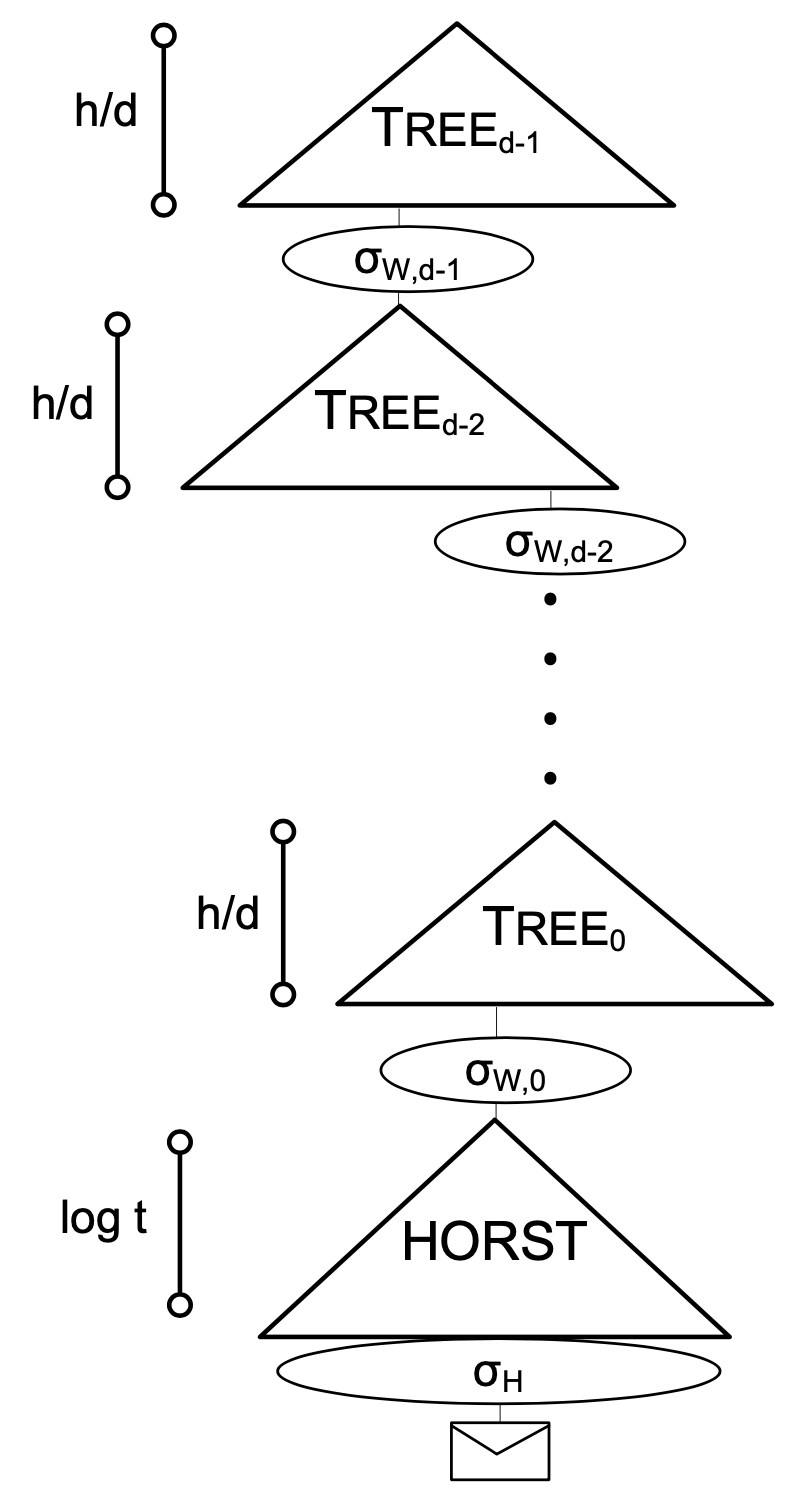
\includegraphics[width=0.4\textwidth]{shpincs_structure.png}
  \caption{Struttura virtuale di una firma SPHINCS}
  \label{fig:shpincs_structure}
\end{figure}

Per facilitare la comprensione, la Figura \ref{fig:sphincs_structure} mostra la struttura virtuale di una firma SPHINCS, cioè di un percorso all'interno dell'ipergrafo. Contiene \(d\) alberi \(TREE_i\) dove \(i \in [d - 1]\) (ognuno dei quali consiste in un albero di hash binario che autentica i nodi radice di \(2^{\frac{h}{d}}\) L-Trees che a loro volta hanno come foglie i nodi delle chiavi pubbliche di una coppia di chiavi WOTS+). Ogni albero autentica l'albero sottostante utilizzando una firma WOTS+ \(\sigma_{W,i}\). L'unica eccezione è \(TREE_0\) che autentica una chiave pubblica HORST utilizzando una firma WOTS+. Infine, la coppia di chiavi HORST viene utilizzata per firmare il messaggio. Quali alberi all'interno dell'ipergrafo vengono utilizzati (il che determina a sua volta le coppie di chiavi WOTS+ utilizzate per la firma) e quale coppia di chiavi HORST è determinata dall'indice generato in modo pseudo-randomiche, non mostrato qui.

Per la generazione pseudo-randomica delle chiavi utilizziamo un semplice schema di indirizzamento. Un indirizzo è una stringa di bit di lunghezza \(a = \lceil \log(d + 1)\rceil + (d - 1)(\frac{h}{d}) + (\frac{h}{d}) = \lceil \log(d + 1)\rceil + h\). L'indirizzo di una coppia di chiavi WOTS+ si ottiene codificando il livello dell'albero a cui appartiene come una stringa di \(\log(d+1)\)-bit (usando \(d-1\) per il livello superiore con un singolo albero). Quindi, si aggiunge l'indice dell'albero nel livello codificato come una stringa di \((d - 1)(\frac{h}{d})\)-bit (si numerano gli alberi da sinistra a destra, partendo da 0 per l'albero più a sinistra). Infine, si aggiunge l'indice della coppia di chiavi WOTS+ all'interno dell'albero, codificato come una stringa di \((\frac{h}{d})\)-bit (anche in questo caso si numera da sinistra a destra, partendo da 0). L'indirizzo della coppia di chiavi HORST si ottiene utilizzando l'indirizzo della coppia di chiavi WOTS+ utilizzata per firmare la sua chiave pubblica e ponendo d come valore di livello nella stringa dell'indirizzo, codificata come stringa di bit \(\lceil \log(d + 1) \rceil\). Per fare un esempio: In SPHINCS-256, un indirizzo ha bisogno di 64 bit.

\subsection{Algoritmo di generazione delle chiavi\\\((SK, PK) \leftarrow kg(1^n)\)}
L'algoritmo di generazione della chiave campiona innanzitutto due valori di chiave segreta \( (SK_1, SK_2) \in \left\{0,1\right\}^n \times \left\{0,1\right\}^n \). Il valore \(SK_1\) viene utilizzato per la generazione di chiavi pseudo-randomiche. Il valore \(SK_2\) è usato per generare un indice imprevedibile nella firma e valori pseudo-randomici per randomizzare l'hash del messaggio nella firma. Inoltre, \(p\) valori casuali uniformi di \(n\)-bit \(Q \overset{\$}{\leftarrow} \left\{0, 1\right\}^{p \times n}\) sono campionati come bitmask, dove \( p = max\left\{w-1, 2(h + \lceil \log l \rceil), 2 \log t\right\} \). Queste bitmaschere sono utilizzate per tutte le istanze WOTS+ e HORST e per gli alberi. Nel seguito utilizzeremo \(Q_{WOTS+}\) per le prime \(w - 1\) bitmaschere (di lunghezza \(n\)) in Q, \(Q_{HORST}\) per le prime \(2 \log t\), \(Q_{L-TREE}\) per le prime \( 2 \lceil \log l \rceil \) e \(Q_{TREE}\) per le \(2h\) stringhe di lunghezza n in Q che seguono \(Q_{L-TREE}\).


\subsection{Algoritmo di firma\\\(\sum \leftarrow sign(M, SK)\)}
Su un messaggio in input \(M \in \left\{0,1\right\}^*\) e una chiave segreta \(SK = \left(SK_1,SK_2,Q\right)\), l'algoritmo di firma calcola un messaggio digest randomizzato \(D \in \left\{0,1\right\}^m\): In primo luogo, viene calcolato uno pseudorandom \(R = (R_1, R_2) \in \left\{0, 1\right\}n \times \left\{0, 1\right\}n\) come viene calcolato \(R \leftarrow F(M, SK_2)\). Quindi, \(D \leftarrow H(R_1,M)\) viene calcolato come hash randomizzato di \(M\) utilizzando i primi \(n\) bit di \(R\) come casualità. Gli ultimi \(n\) bit di \(R\) sono utilizzati per selezionare una coppia di chiavi HORST, calcolando un indice di \(h\) bit \(i \leftarrow CHOP(R_2 , h)\) come il primo \(h\) bit di \(R_2\).

Dato un indice \(i\), la coppia di chiavi HORST con indirizzo \((d\|i(0, (d - 1)\frac{h}{d})||i((d - 1)\frac{h}{d}, \frac{h}{d}))\) viene usato per firmare il messaggio digest D, cioè, i primi \((d - 1)\frac{h}{d}\) bit di \(i\) sono usati come indice dell'albero e i restanti bit per l'indice all'interno dell'albero.

La firma SPHINCS \( \sum(i, R_1, \sigma_H, \sigma_W,0, AUTH_{A_0} , . . . , \sigma_W,d-1, AUTH_{A_{d-1}}) \) contiene oltre all'indice \(i\), la casualità \(R_1\) e alla firma HORST \(\sigma_H\) anche una firma WOTS+ e un percorso di autenticazione \(\sigma_W,i, AUTH_{A_i} , dove \; i \in [d-2]\) per livello. Questi sono calcolati come segue: La coppia di chiavi WOTS+ con indirizzo \(A_0\) viene utilizzata per firmare \(pk_H\), dove \(A_0\) è l'indirizzo ottenuto prendendo \(A_{HORST}\) e impostando i primi \(\lceil \log(d + 1)\rceil\) bit a zero. Questo viene fatto eseguendo \(\sigma_{W,1} \leftarrow (pk_H, S_{A_0} , Q_{WOTS+} )\) utilizzando le maschere di bit di WOTS+. Quindi viene calcolato il percorso di autenticazione \(AUTH_i((d-1)\frac{h}{d},\frac{h}{d}))\) della coppia di chiavi WOTS+ utilizzata. Quindi, la chiave pubblica WOTS+ \(pk_{W,0}\) viene calcolata eseguendo \\ \(pk_{W,0} \leftarrow WOTS.vf(pkH, \sigma_W, 0, QWOTS+)\). Il nodo radice \(ROOT_0\) dell'albero viene calcolato comprimendo prima \(pk_{W,0}\) con un L-Tree. Quindi si applica l'algoritmo che, data una foglia \(L_i\) insieme al suo percorso di autenticazione \(AUTH_i\), calcola la radice dell'albero utilizzando, in questo caso, l'indice della coppia di chiavi WOTS+ all'interno dell'albero, la radice dell'L-Tree e \(AUTH_i((d-1)\frac{h}{d},\frac{h}{d}))\).

Questa procedura viene ripetuta dal livello 1 al livello \(d - 1\) con le due seguenti differenze: Su livello \( 1 \leqslant j < \), WOTS+ viene usato per firmare \(ROOT_{j-1}\), la radice calcolata al termine dell'iterazione precedente.

L'indirizzo della coppia di chiavi WOTS+ usata sul livello \(j\) viene calcolata come \( A_j = (j\|i(0, (d - 1 - j)\frac{h}{d})\|i((d - 1 - j)\frac{h}{d}, \frac{h}{d})) \), cioè su ogni livello gli ultimi \((\frac{h}{d})\) bit dell'indirizzo dell'albero diventano il nuovo indirizzo della foglia e i bit rimanenti del precedente indirizzo dell'albero diventano il nuovo indirizzo dell'albero.

Infine, la funzione di firma restituisce in output:
\[ \sum = (i, R_1, \sigma_H, \sigma_W,0, AUTH_{A_0} , . . . , \sigma_{W,d-1}, AUTH_{A_{d-1}} ) \]

\subsection{Algoritmo di verifica\\\(b \leftarrow vf(M, \sum, PK)\)}
Su un messagio in input \( M \in \left\{0,1\right\}^* \), una firma \(\Sigma\), e una chiave pubblica PK, l'algoritmo calcola il messaggio digest \( D \leftarrow H(R_1,M) \) usando un \(R_1\) randomico contenuto nella firma. Il messaggio digest \(D\) e la maschera di bit HORST, definita come \(Q_{HORST}\), sono usate per calcolare la chiave pubblica HORST \( pk_H \leftarrow HORST.vf(D, \sigma_H, Q_{HORST}) \) dalla firma HORST. Se \(HORST.vf\) fallisce, allora la verifica restituirà \textit{false}. La chiave pubblica HORST viene a sua volta utilizzata insieme alle maschere di bit WOTS+ e alla firma WOTS+ per calcolare la prima chiave pubblica WOTS+ \(pk_{W,0} \leftarrow WOTS.vf(pk_H, \sigma_{W,0}, Q:{WOTS+})\). Un L-Tree viene utilizzato per calcolare \(L_i((d-1)\frac{h}{d},\frac{h}{d})\), la foglia corrispondente a \(pk_{W,0}\). Quindi, la radice \(Root_0\) del rispettivo albero viene calcolata utilizzando l'algoritmo che calcola la radice eseguendolo con l'indice \(i((d - 1)\frac{h}{d}, \frac{h}{d})\), la foglia \(L_i((d-1)\frac{h}{d},\frac{h}{d})\) e il percorso di autenticazione \(Auth_0\).

Poi, questa procedura viene ripetuta per gli strati da \(1\) a \(d - 1\) con le due seguenti differenze. In primo luogo, sul livello \(1 \leqslant j < d\) viene utilizzata la radice dell'albero \(Root_{j-1}\) precedentemente elaborato per calcolare la chiave pubblica WOTS+ \(pk_{W,j}\). In secondo luogo, la foglia calcolata da \(pk_{W,j}\) utilizzando un albero a \(L\) è \(L_{i((d-1-j)\frac{h}{d},\frac{h}{d})}\), cioè l'indice della foglia all'interno dell'albero può essere calcolato tagliando gli ultimi \(j(\frac{h}{d})\) bit di \(i\) e quindi utilizzando gli ultimi \(\frac{h}{d}\) bit della stringa di bit risultante.

Il risultato dell'iterazione finale sullo strato \(d - 1\) è un valore \(Root_{d-1}\) per il nodo radice del singolo albero sullo strato superiore. Questo valore viene confrontato con il primo elemento della chiave pubblica, ovvero \(PK_1 \overset{?}{=} Root_{d-1}\). Se il confronto è valido, vf restituisce \textit{true}, altrimenti restituisce \textit{false}.